\chapter{Ganiw}

\section{Introduction}

TODO: Introduction sur les botnets

Le \textit{sample} porté à l'étude porte le doux nom de \textbf{Ganiw} mais est
aussi connu sous les nom de \textbf{BillGates} ou de combinaisons comme
\textbf{LINUX.BACKDOOR.GATES}.\\
TODO:md5/sha1\\
Celui-ci semble avoir été étudié pour la première fois en février 2014
sur un site russe: \textit{\href{https://habrahabr.ru/post/213973/}
{Studying the BillGates Linux Botnet}}\footnotemark,
mais continue tout de même à être étudié et à être actif.
En effet, comme il sera expliqué plus amplement par la suite, celui-ci présente
des propriétés particulières.\\

Ce malware est présent uniquement sur les systèmes Linux.
Ce qui n'est pas anodin et sans lien quand à son utilisation: le
développement toujours plus important des objets connectés dans l'IoT
en fait une cible de choix. Linux ou les systèmes basés sur son noyau
(comme avec le projet Yocto\footnotemark) sont donc
des RTOS parfaits (TODO à reformuler) pour de petits appareils
car légers et open-sources et y ont le monopole.
De plus, ces objets connectés sont, en règle générale, peu protégés
(absence de firewall, mots de passe faibles,\ldots)
et non surveillés ou peu maintenus.
Ce sont donc des cibles de choix pour un malware de type \textit{BotNet},
comme \textbf{Ganiw}, pour mener des attaques réseaux de types DDOS par exemple.\\

La suite de cette étude va se faire sous 2 formes: une partie par
analyse statique du binaire et une autre par analyse dynamique,
permettant de confirmer et approfondir les données recueillies précédemment.

\footnotetext{Traduit depuis le russe}
\footnotetext{\url{https://www.yoctoproject.org/}}

\section{Étude -- Analyse statique}

\subsection{Outils d'analyse}

TODO: description outils et buts d'analyse statique

Contrairement à l'analyse statique dans son ensemble,
le travail effectué ne va pas chercher à debugger le programme
ou à y trouver les erreurs de programmation.
Le but, dans cette partie, va être d'obtenir des informations sur le
comportement du binaire lors de son exécution sans réellement l'exécuter.
N'ayant bien souvent que le binaire à disposition, l'étude se portera donc
sur du code asm (TODO: à reformuler) ou du code compilé,
en fonction des outils mis à disposition de l'analyste.\\

Ici, le travail de rétro-ingénierie se fera à partir du code assembleur et ce,
car aucun décompilateur (comme
\href{https://www.hex-rays.com/products/decompiler/}
{\textit{Hex-Rays Decompiler}}) n'était à disposition.
Les outils utilisés seront donc le debugger GNU
\href{https://www.sourceware.org/gdb/}{\textit{GDB}} et le désassembleur
\href{https://github.com/radare/radare2}{\textit{Radare2}},
qui sont tous les deux des logiciels libres.\\
TODO: parler du C++, not stripped

Afin de mieux suivre le fonctionnement et l'étude, pas à pas, de ce malware, une figure récapitulative de son comportement est présentée ici: fig~\ref{recap}.

\begin{figure}[!h]

  \centering
  \begin{tikzpicture}

  \node[draw, minimum width=2cm, text width=2cm, text centered]
  (Be) at (0,0) {Beikong\\BillGates};
  \node[draw, minimum width=2cm, text width=2cm, text centered]
  (Ba) at (5,0) {Backdoor\\Getty};
  \node[draw, minimum width=2cm, text width=2cm, text centered]
  (Mo) at (2,-2.5) {Monitor\\.sshd};
  \node[draw, text centered, shape=diamond]
  (Ta) at (9.5,1.7) {Target};
  \node[draw, minimum width=2cm, text width=2cm, text centered]
  (Us) at (9,-3) {User};
  \node[draw, minimum width=2cm, text width=2cm, text centered]
  (Sy) at (9,-4) {Systool};
  \node[draw, minimum width=2cm, text width=2cm, text centered]
  (OS) at (9,-5.5) {Original\\Systool};
  \node[draw, cloud, cloud puffs=11, minimum height=.5cm,
    minimum width=1.5cm] (CC1) at (0,5) {\shortstack{C\&C}};
  \node (IP) at (-1,6.1) {\shortstack{115.28.206.48:25000}};
  \node[draw, cloud, cloud puffs=11, minimum height=.5cm,
    minimum width=1.5cm] (CC2) at (4.8,5) {\shortstack{C\&C}};
  \node (IP) at (4.5,6.1) {\shortstack{www.i0cc.com}};
  \node[draw, cloud, cloud puffs=11, minimum height=1cm,
    minimum width=1cm] (US) at (2.5,3) {\shortstack{\scriptsize Update\\\scriptsize Server}};

  \draw[-] plot [smooth, tension=0.5] coordinates {(10,-1.8) (7.75,-2.3) (7.75,-6.2) (10,-6.8)};
  \node (Ca) at (9,-7.2) {\shortstack{Cach\'e à\\l'utilisateur}};
  \draw[->, >=latex, thick, color=black!60!green] (Ba.-5) to[bend left]
  node[midway, color=black!60!green, xshift=1.4cm, yshift=.2cm] {\shortstack{Installe sur\\le PC infect\'e}} (9,-1.8);

  \draw[<->, >=latex, color=blue!50!black] (CC1) -- (Be)
  node[midway, xshift=-1.4cm, yshift=.2cm]
  {\shortstack{Communique\\et \'echange\\des informations}};

  \draw[<->, >=latex, color=blue!50!black] (CC2) -- (Ba.115)
  node[midway, xshift=1.4cm, yshift=.7cm]
  {\shortstack{Communique\\et \'echange\\des informations}};

  \draw[<->, >=latex] (US) -- (Ba);
  \draw[<->, >=latex] (US) -- (Be)
  node[midway, xshift=1.3cm, yshift=.2cm]
  {\shortstack{Mise à jour}};

  \draw[->, >=latex, thick, color=black!60!green] (Be.-120) -- (Mo.120)
  node[midway, xshift=-.8cm, yshift=-.2cm, color=black!60!green]
  {\shortstack{Installe\\et lance}};

  \draw[->, >=latex, dashed] (Mo.80) -- (Be.-80)
  node[midway, xshift=2.2cm, yshift=-.2cm]
  {\shortstack{Surveille\\le comportement}};

  \draw[->, >=latex, thick, color=black!60!green] (Be.10) -- (Ba.170)
  node[midway, yshift=.5cm, color=black!60!green]
  {\shortstack{Installe\\et lance}};

  \draw[->, >=latex] (Be.-10) -- (Ba.-170)
  node[midway, yshift=-.3cm]
  {\shortstack{Commande}};

  \draw[->, >=latex, thick, double, red] (Ba.north) to[bend left]
  node[midway, xshift=.7cm, yshift=-.7cm, red]
  {\shortstack{Attaques}}(Ta.120);

  \draw[->, >=latex, double, red] (Ba.70) to[bend left] (Ta.135);
  \draw[->, >=latex, double, dashed, red] (Ba.55) to[bend left] (Ta.150);

  \draw[->, >=latex] (Us.-110) to[bend right] (Sy.105);
  \draw[->, >=latex] (Sy.70) to[bend right] (Us.-70);
  \draw[->, >=latex] (Sy.-105) to[bend right] (OS.100);
  \draw[->, >=latex] (OS.75) to[bend right] (Sy.-70);

\end{tikzpicture}

  \label{recap}
  \caption{Fonctionnement schématique de Ganiw}

\end{figure}

\subsection{Étude -- Main}

Le point d'entrée du binaire se fait au niveau de la fonction \textit{main}. Sans trop entrer dans les détails, il est aisé de remarquer la structure modulaire du malware~\ref{modulaire}.\\

\begin{figure}[!h]

  \centering
  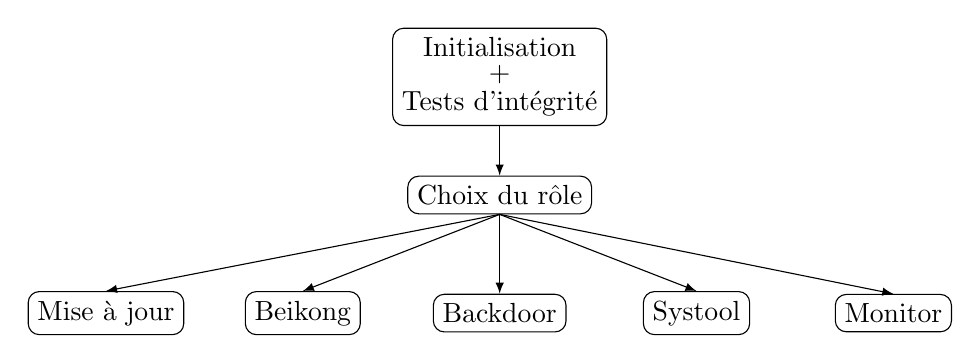
\begin{tikzpicture}

  \node[draw, rounded corners] (In) at (0,3)
       {\shortstack{Initialisation\\+\\Tests d'int\'egrit\'e}};
  \node[draw, rounded corners] (Cx) at (0,1.5) {\shortstack{Choix du r\^ole}};
  \node[draw, rounded corners] (MJ) at (-5,0) {\shortstack{Mise \`a jour}};
  \node[draw, rounded corners] (Be) at (-2.5,0) {\shortstack{Beikong}};
  \node[draw, rounded corners] (Ba) at (0,0) {\shortstack{Backdoor}};
  \node[draw, rounded corners] (Sy) at (2.5,0) {\shortstack{Systool}};
  \node[draw, rounded corners] (Mo) at (5,0) {\shortstack{Monitor}};

  \draw[->, >=latex] (In) to (Cx);
  \draw[->, >=latex] (Cx.-90) to (MJ.90);
  \draw[->, >=latex] (Cx.-90) to (Be.90);
  \draw[->, >=latex] (Cx.-90) to (Ba.90);
  \draw[->, >=latex] (Cx.-90) to (Sy.90);
  \draw[->, >=latex] (Cx.-90) to (Mo.90);

\end{tikzpicture}

  \label{modulaire}
  \caption{Modules mis à disposition du malware}

\end{figure}

La fonction main commence donc par un ensemble de tests et d'initialisation de variables, de mises en place du système.\\
\subsubsection{Close all files descriptor}
Tout d'abord, le malware va fermer tous les points d'entrées ou de sorties sur/depuis lui, exceptés ceux standards (stdin, stdout et stderr).
\subsubsection{Decode and init first variables set}
La deuxième partie consiste en l'initialisation de certaines variables globales au programme, depuis une chaîne de caractères quelque peu étrange. Dans le sample étudié, celle-ci correspond à: \\"681A1C1543072E0140491F162F0B55545C55775F55565E57745E5D545652705D5E55585F70585C5659577D5\\C5F565C0423575B025A51720A56".\\
Une fonction de décodage, avec le mot clef 'Google', est appliquée à cette chaîne. Le code C++ associé est présent en annexes~\ref{C++}. Les informations obtenues sont alors stockées dans des flags (figure~\ref{first_flag}), qui serviront à définir le comportement futur du binaire.

\begin{figure}[h!]
  \centering
  \begin{tabular}{|l|c|l|c|}
    \hline
    \multicolumn{1}{|l|}{\cellcolor{gray!20} g\_Iud77} & \multicolumn{3}{c|}{681A1C154 [\ldots] 0423575B025A51720A56} \\
    \hline
    \cellcolor{gray!20} g\_strMonitorFile & /usr/bin/.sshd & \cellcolor{gray!20} g\_uHiddenPt & 30000 \\
    \hline
    \cellcolor{gray!20} g\_iFileSize & 1223123 & \cellcolor{gray!20} g\_iHardStart & 772124 \\
    \hline
    \cellcolor{gray!20} g\_iSoftStart & 773152 & \cellcolor{gray!20} g\_strDoFun & 3010ad84e645e9 \\
    \hline
  \end{tabular}
  \caption{Valeurs des premiers flags initialisés}
  \label{first_flag}
\end{figure}

\subsubsection{Get module full path}

Ensuite, le chemin absolu du binaire va être récupéré à l'aide de l'appel système \textit{readlink} et du fichier \textit{$\backslash$proc$\backslash$\textbf{XX}$\backslash$exe} où \textit{\textbf{XX}} correspond au pid du processus courant.

\subsubsection{Integrity check}

Un test d'intégrité va être effectué à cette étape. La taille de l'exécutable va être récupérée à l'aide de l'appel système \textit{stat} et va être comparée au flag défini un peu plus tôt: \textit{g\_iFileSize}. Si les deux tailles sont différentes, alors le binaire fera une erreur de segmentation.

\subsubsection{Get Parent Path}

Puis, le chemin absolu vers le processus père de l'exécutable est récupéré, de la même manière que précédemment, mais avec la fonction \textit{getppid}.

\subsubsection{Anti-debug protection}

Un test est de nouveau effectué, mais, cette fois-ci, afin d'"empêcher" le débuggage du malware. Si le mot clef "gdb" est présent dans le chemin absolu du père, alors, le binaire fera une erreur de segmentation.

\subsubsection{Second variables set initialization}

La deuxième série d'initialisation de variables n'est pas obfusquée: les noms de variables et leurs contenus sont présentés dans le tableau suivant (figure~\ref{second_flag}).

\begin{figure}[h!]
  \centering
  \begin{tabular}{|l|c|l|c|}
    \hline
    \cellcolor{gray!20} g\_strSN & DBSecuritySpt & \cellcolor{gray!20} g\_strML & /tmp/moni.lod \\
    \hline
    \cellcolor{gray!20} g\_strBDSN & selinux & \cellcolor{gray!20} g\_strGL & /tmp/gates.lod \\
    \hline
    \cellcolor{gray!20} g\_strBDG & getty & \multicolumn{2}{c|}{}\\
    \hline
  \end{tabular}
  \caption{Valeurs des seconds flags initialisés}
  \label{second_flag}
\end{figure}

\subsubsection{Check of gates type}

Cette étape va définir le comportement du binaire, en fonction de son chemin absolu. En effet, celui-ci va être comparé au différentes valeurs présentes dans les flags définis plus tôt, afin de définir le contenu d'un nouveau flag: \textit{g\_iGatesType} (voir figure~\ref{gates_type}). TODO: comportement uaSystools\\

\begin{algorithm}[H]
  \label{gates_type}
  \caption{Initialisation du flag g\_iGatesType}
  \begin{algorithmic}[1]

    \State {path := GetModuleFullPath}
    \State {uaSystools := ['/bin/netstat', '/bin/lsof', '/bin/ps', '/bin/ss', \\
        \ \ \ \ \ \ \ \ \ \ \ \ \ \ \ \ \ \ \ \ '/usr/bin/netstat','/usr/bin/lsof', '/usr/bin/ps', '/usr/bin/ss',\\
        \ \ \ \ \ \ \ \ \ \ \ \ \ \ \ \ \ \ \ \ '/usr/sbin/netstat', '/usr/sbin/lsof', '/usr/sbin/ps', '/usr/sbin/ss']}
    \State {}
    \If {(path = g\_strMonitorFile)} \State {g\_iGatesType := 0} \Comment Module MainMonitor
    \Else
    \If {(path = "/usr/bin/bsd-port/getty")} \Comment Issu de g\_strBDG \State {g\_iGatesType := 2} \Comment Module MainBackdoor
    \Else
    \If {(path $\in$ uaSystools)} \State {g\_iGatesType := 3} \Comment Module MainSystool
    \Else \State {g\_iGatesType := 1} \Comment Module MainBeikong
    \EndIf \EndIf \EndIf

  \end{algorithmic}
\end{algorithm}

\subsubsection{Decode and init third variables set}

Tout comme lors de l'étape \textbf{Decode and init first varaibles set}, un ensemble de variables va être initialisé en fonction d'une valeur, rentrée en clair dans le binaire. Ici, celle-ci sera plus grande et a pour valeur:\\
TODO: explication + code C++""\\

\begin{figure}[h!]
  \centering
  \begin{tabular}{|l|c|l|c|}
    \hline
    \multicolumn{1}{|l|}{\cellcolor{gray!20} g\_Iud76} & \multicolumn{3}{c|}{[\ldots]} \\
    \hline
    \cellcolor{gray!20} g\_strConnTgts & 115.231.168.64 & \cellcolor{gray!20} g\_iIsService & 1 \\
    \hline
    \cellcolor{gray!20} g\_iGatsPort & 13864 & \cellcolor{gray!20} g\_strForceNote & ssh4ckss \\
    \hline
    \cellcolor{gray!20} g\_iGatsFx & 1 & \cellcolor{gray!20} g\_iDoBackdoor & 1 \\
    \hline
  \end{tabular}
  \caption{Valeurs des derniers flags initialisés}
  \label{third_flag}
\end{figure}

\subsubsection{Module choice}

Enfin, le malware va charger un des modules, en fonction de la valeur du flag \textit{g\_iGatesType}, ou se mettre à jour si cela est possible.\\

Le pseudo-code de la fonction main, ainsi que de chacunes de ses étapes, est présent en annexes~\ref{main_algo}.\\

\subsection{Étude -- Beikong/Bill}

Le module Beikong (ou Bill) est le module d'installation mais également le premier module principal du botnet. Son rôle est, d'abord, de nettoyer le système en arrêtant et supprimant les potentielles instances de lui-même qui tournerait déjà sur le système, puis de mettre en place le démarrage automatique de son exécutable au lancement du système et, enfin, de réinstaller et démarrer les modules Backdoor et Monitor. Il communique également avec un serveur C\&C.
\newline

Pseudo-code :
\begin{itemize}
\item Arrête le module Monitor
\item Arrête le module Bill
\item Si la configuration le précise (booléen IsService à Vrai), créer un script i\textbf{/etc/init.d/DbSecuritySpt} et des liens symboliques \textbf{/etc/rc$i$.d/S97DbSecuritySpt} (avec $i$ allant de 1 à 5) vers ce script, permettant de lancer l'exécutable actuel au démarrage
\item Si la configuration le précise (booléen DoBackdoor à Vrai), arrête le module Backdoor et le réinstalle (dans \textbf{/usr/bin/bsd-port/getty}) et le relance
\item Si l'exécutable est exécuté en tant que root, indique la localisation du fichier du module Beikong dans \textbf{/tmp/notify.file} et installe/lance le module Monitor (dans \textbf{/usr/bin/.sshd})
\item Exécute MainProcess()
\end{itemize}

%Depuis le main, HGrd9 écrit DbSecuritySpt (g\_strSN), selinux (g\_strBSDN), getty (g\_strBDG), /tmp/moni.lod (g__strML), (g__strGL) avec 'nkfsd8' qui écrit tmp, 'Kusdf9' qui écrit moni, tRd76 qui écrit lod. KDS87y inutil !! 0sdku6 '/tmp/moni.lod'
%\\

\subsection{Étude -- Backdoor}
Le module Backdoor est le deuxième module principal du botnet. Il s'occupe de remplacer quelques outils systèmes classiques par son exécutable pour cacher ses traces. Il communique lui aussi avec un serveur C\&C.\newline

Pseudo-code :
\begin{itemize}
\item Inscrit le pid du processus actuel dans le fichier \textbf{/usr/bin/bsd-port/getty.lock} et lock le fichier
\item Créer un script \textbf{/etc/init.d/selinux} et des liens symboliques \textbf{/etc/rc$i$.d/S99selinux} (avec $i$ allant de 1 à 5) vers ce script, permettant de lancer l'exécutable actuel (\textbf{/usr/bin/bsd-port/getty}) au démarrage
\item Copie et remplace les outils systèmes $netstat$, $lsof$, $ps$ et $ss$ dans les dossiers \textbf{/bin/}, \textbf{/usr/bin/} et \textbf{/usr/sbin/}
\item Exécute MainProcess()
\end{itemize}

\subsection{Étude -- MainProcess, Attaques et communication C\&C}
Dans les modules précédents on finit dans les deux cas par exécuter la fonction MainProcess(). Cette fonction constitue la partie active du botnet.\newline

Pseudo-code de MainProcess :
\begin{itemize}
\item Initialise DNSCache (parse \textbf{/etc/resolv.conf}, utilisé pour la résolution de noms de domaine)
\item Initialise ConfigDoing (parse \textbf{conf.n} qui se trouve dans le dossier courant)
\item Initialise CmdDoing (parse \textbf{cmd.n} qui se trouve dans le dossier courant)
\item Initialise StatBase (GetOS, GetCpuSpd, CpuUse, NetUse, GetMemSize)
\item Initialise ProvinceDns (liste de DNS utilisés pour l'amplification)
\item Essaye de charger \textbf{/usr/lib/xpacket.ko} avec system("insmod /usr/lib/xpacket.ko")
\item Initialise CAmpResource (en lisant le fichier \textbf{/usr/lib/libamplify.so})
\item Initialise CManager (démarrage des threads principaux et de la communication au C\&C)
\end{itemize}

\subsubsection{Communication avec le serveur C\&C}
Le botnet à besoin de communiquer avec un ou plusieurs serveurs C\&C pour pouvoir agir.
La communication au C\&C peut se faire dans les deux sens : soit le client se connecte au serveur C\&C, soit le serveur C\&C se connecte au client. Le choix est fait en fonction du paramètre de configuration g\_GatsIsFx; dans notre cas le client se connecte au serveur (ce qui est préférable étant donné que beaucoup de routeurs font du NAT par défaut, ce qui empêche les connections sur des ports arbitraires depuis l'extérieur).\newline

Dans le cas où g\_iGatsIsFX est vrai, un thread "ThreadFXConnection" est crée pour gérer chaque connection aux différents serveurs C\&C
La communication s'effectue par le biais d'une ou plusieurs connections TCP/IP en direction des IPs et du port définis dans g\_strConnTgts et g\_iGatsPort respectivement.\newline

C'est ensuite le thread "ThreadTaskGates" s'occupe de faire ce que demande le serveur C\&C. Il vérifie d'abord si des commandes ont été reçues et si c'est le cas, exécute le handler associé, puis recommence indéfiniement.\newline
Plusieurs commandes sont disponibles :
\begin{itemize}
\item Commande \#1 : Démarrer une attaque sur une ou plusieurs cibles
\item Commande \#2 : Arrêter les attaques ou mises à jour en cours
\item Commande \#3 : Modifier la configuration du module
\item Commande \#5 : Démarrer une mise à jour du client
\item Commande \#7 : Modifie la cmd actuelle (??)
\item Commande \#8 : DoFakeDetect (??)
\item Commande \#9 : Demander l'accès à un reverse shell en tant que root sur le client
\end{itemize}

\subsubsection{Attaques normales}
TODO
\subsubsection{Attaques noyaux}
TODO

\subsection{Étude -- Autres modules}
\subsubsection{Monitor}
Le module Monitor s'occupe de vérifier que le module Bill reste en vie, et de le relancer si il ne l'est plus.

Pseudo-code :
\begin{itemize}
\item Écrit le pid du processus actuel dans le fichier \textbf{/tmp/moni.lod} et lock le fichier
\item Récupère la localisation du fichier Beikong dans \textbf{/tmp/notify.file} et supprime le fichier
\item Démarre un thread "CThreadMonGates" qui vérifie, toutes les 60 secondes, que le fichier \textbf{/tmp/gates.lock} à un lock actif (et donc que le module Bill est toujours vivant) et relance le module Bill si ce n'est pas le cas
\item Boucle à l'infini
\end{itemize}

\subsubsection{Systool}
Le module Systool est le module qui s'exécute lorsque l'exécutable se trouve à la place d'un des outils systèmes $netstat$, $lsof$, $ps$ ou $ss$. Son rôle est de filtrer les sorties des outils qu'il remplace pour cacher les parties qui révèlent la présence du module Backdoor.\newline

Pseudo-code :
\begin{itemize}
\item Déduit le chemin de l'outil système original associé, en le dérivant du nom de l'exécutable actuel
\item Si l'outil a été trouvé, on récupère le chemin complet de l'exécutable du module Backdoor ainsi que la valeur du HiddenPort, on exécute l'outil système avec les arguments passés en paramètres et on filtre la sortie en n'affichant pas les références aux chemin et port récupérer précédemment
\end{itemize}

\subsubsection{Update}
La partie mise à jour du botnet est composée de deux morceaux : un premier morceau qui est le handler de la commande $DoUpdateCommand$ qui peut être envoyée par le serveur C\&C et une deuxième partie qui fonctionne comme les modules précédents, dans le sens où, si l'exécutable porte le nom \textbf{update\_temporary}, alors il exécute la méthode $DoUpdate$ et se termine ensuite.

Pseudo-code DoUpdateCommand :
\begin{itemize}
\item Méthode 1 : Download, move to libamplify.so, ReinitReadResources (libamplify.so)
\item Méthode 5 : Copy self, execute (update\_temporary, executes DoUpdate)
\item Méthode 4 : Download, move, execute if needed
\end{itemize}

Pseudo-code DoUpdate :
\begin{itemize}
\item Si argc == 5, on prépare une update pour cfg1
\item Si atoi(argv[1] == 5) (cas principal), on modifie le fichier argv[3] en HardStart et SoftStart
\end{itemize}

\section{Étude -- Analyse dynamique}

inetsim gdb strace wireshark/tcpdump ++ mise en place vm/dns server/...

Mise en place d'un environnement de travail $+$ outils utilisés (lemon ?)\\
→ crontab trouvé dans l'analyse statique --> fonctionnement fichier rc.

\section{Conclusion}
